%---------------------------------------------------------------------------------------------------
% Introduction
%---------------------------------------------------------------------------------------------------
\newpage
%\part{start}
\chapter{Introduction}
	\section{Problem Statement}
		The main objective that I had to accomplish for the navigation module was, to connect the google direction API \cite{googleDirecAPI}. 
		This sub-module is responsible for sending queries based upon users current location and the end destination. 
		The queries will be resolved in the state of the art google servers where the 
		routes will be calculated using advanced algorithms and the massive amount of data that google possess. 

		\begin{figure}[htbp!]
			\centering 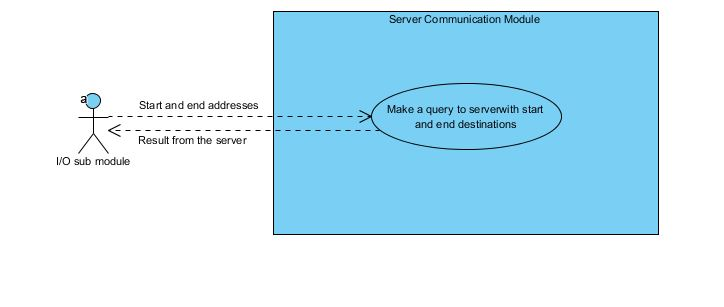
\includegraphics[scale=0.65]{grafiken/googleServerCommunication.jpg}
			\caption{Use case diagram: Google API sub-module communication}
			\label{fig:Google API communication}
		\end{figure}

	\par
		From the figure \ref{fig:Google API communication} it can be a seen that the API sub-module is 
		just an interface which communicates with the server to provide the calculated is a 
		middleware between the server and the navigation.

	\section{Motivation}
		The major focus of my objectives were related to the software engineering aspects instead of
		the hardware side. I believe that software design is an important part of every project and
		it has always been a challenge to design a project base
		in a way which is robust, scalable and can be maintained with ease. By choosing this package,
		I had the flexibility to develop a system by applying the software design patterns and experiment with 
		the new	technologies available and see them in practice including, what are their pros and cons. 

	\section{Report Overview}
		Here is a brief outline, providing a short description on what each chapter contains, to get an
		quick overview of the my report.
		
		\paragraph{Chapter 2: "Requirement Analysis"}
			this chapter describes the functional and non-functional objectives of the sub-module. 
		\paragraph{Chapter 3: "Sofware Design"}
			this chapter explains in detail, how the navigation modules software architecture is designed. 
		\paragraph{Chapter 4: "Implementation"} 
			this chapter is where the details of the Implementation decisions and the manual how to understand 
			the project lies.
		\paragraph{Chapter 5: "Testing and Result"}
			this chapter shows the result for the Google Direction API and for some test cases to ensure what 
			a proper error handling. 
		\paragraph{Chapter 6: "Conclusion"} 
			presents the outcomes and what were the things which could not be completed and some improvements
			which can be done for the future.
